% Intégration des figures - Tests de Riemann et Convergence
% Sprint 2 - Niveau 1 (Fondations Mathématiques)
% Date: 17 octobre 2025
% Format: PNG (300 DPI) pour compatibilité LaTeX

% Figure 7.1: Test de choc simple (motos)
\begin{figure}[h!]
\centering
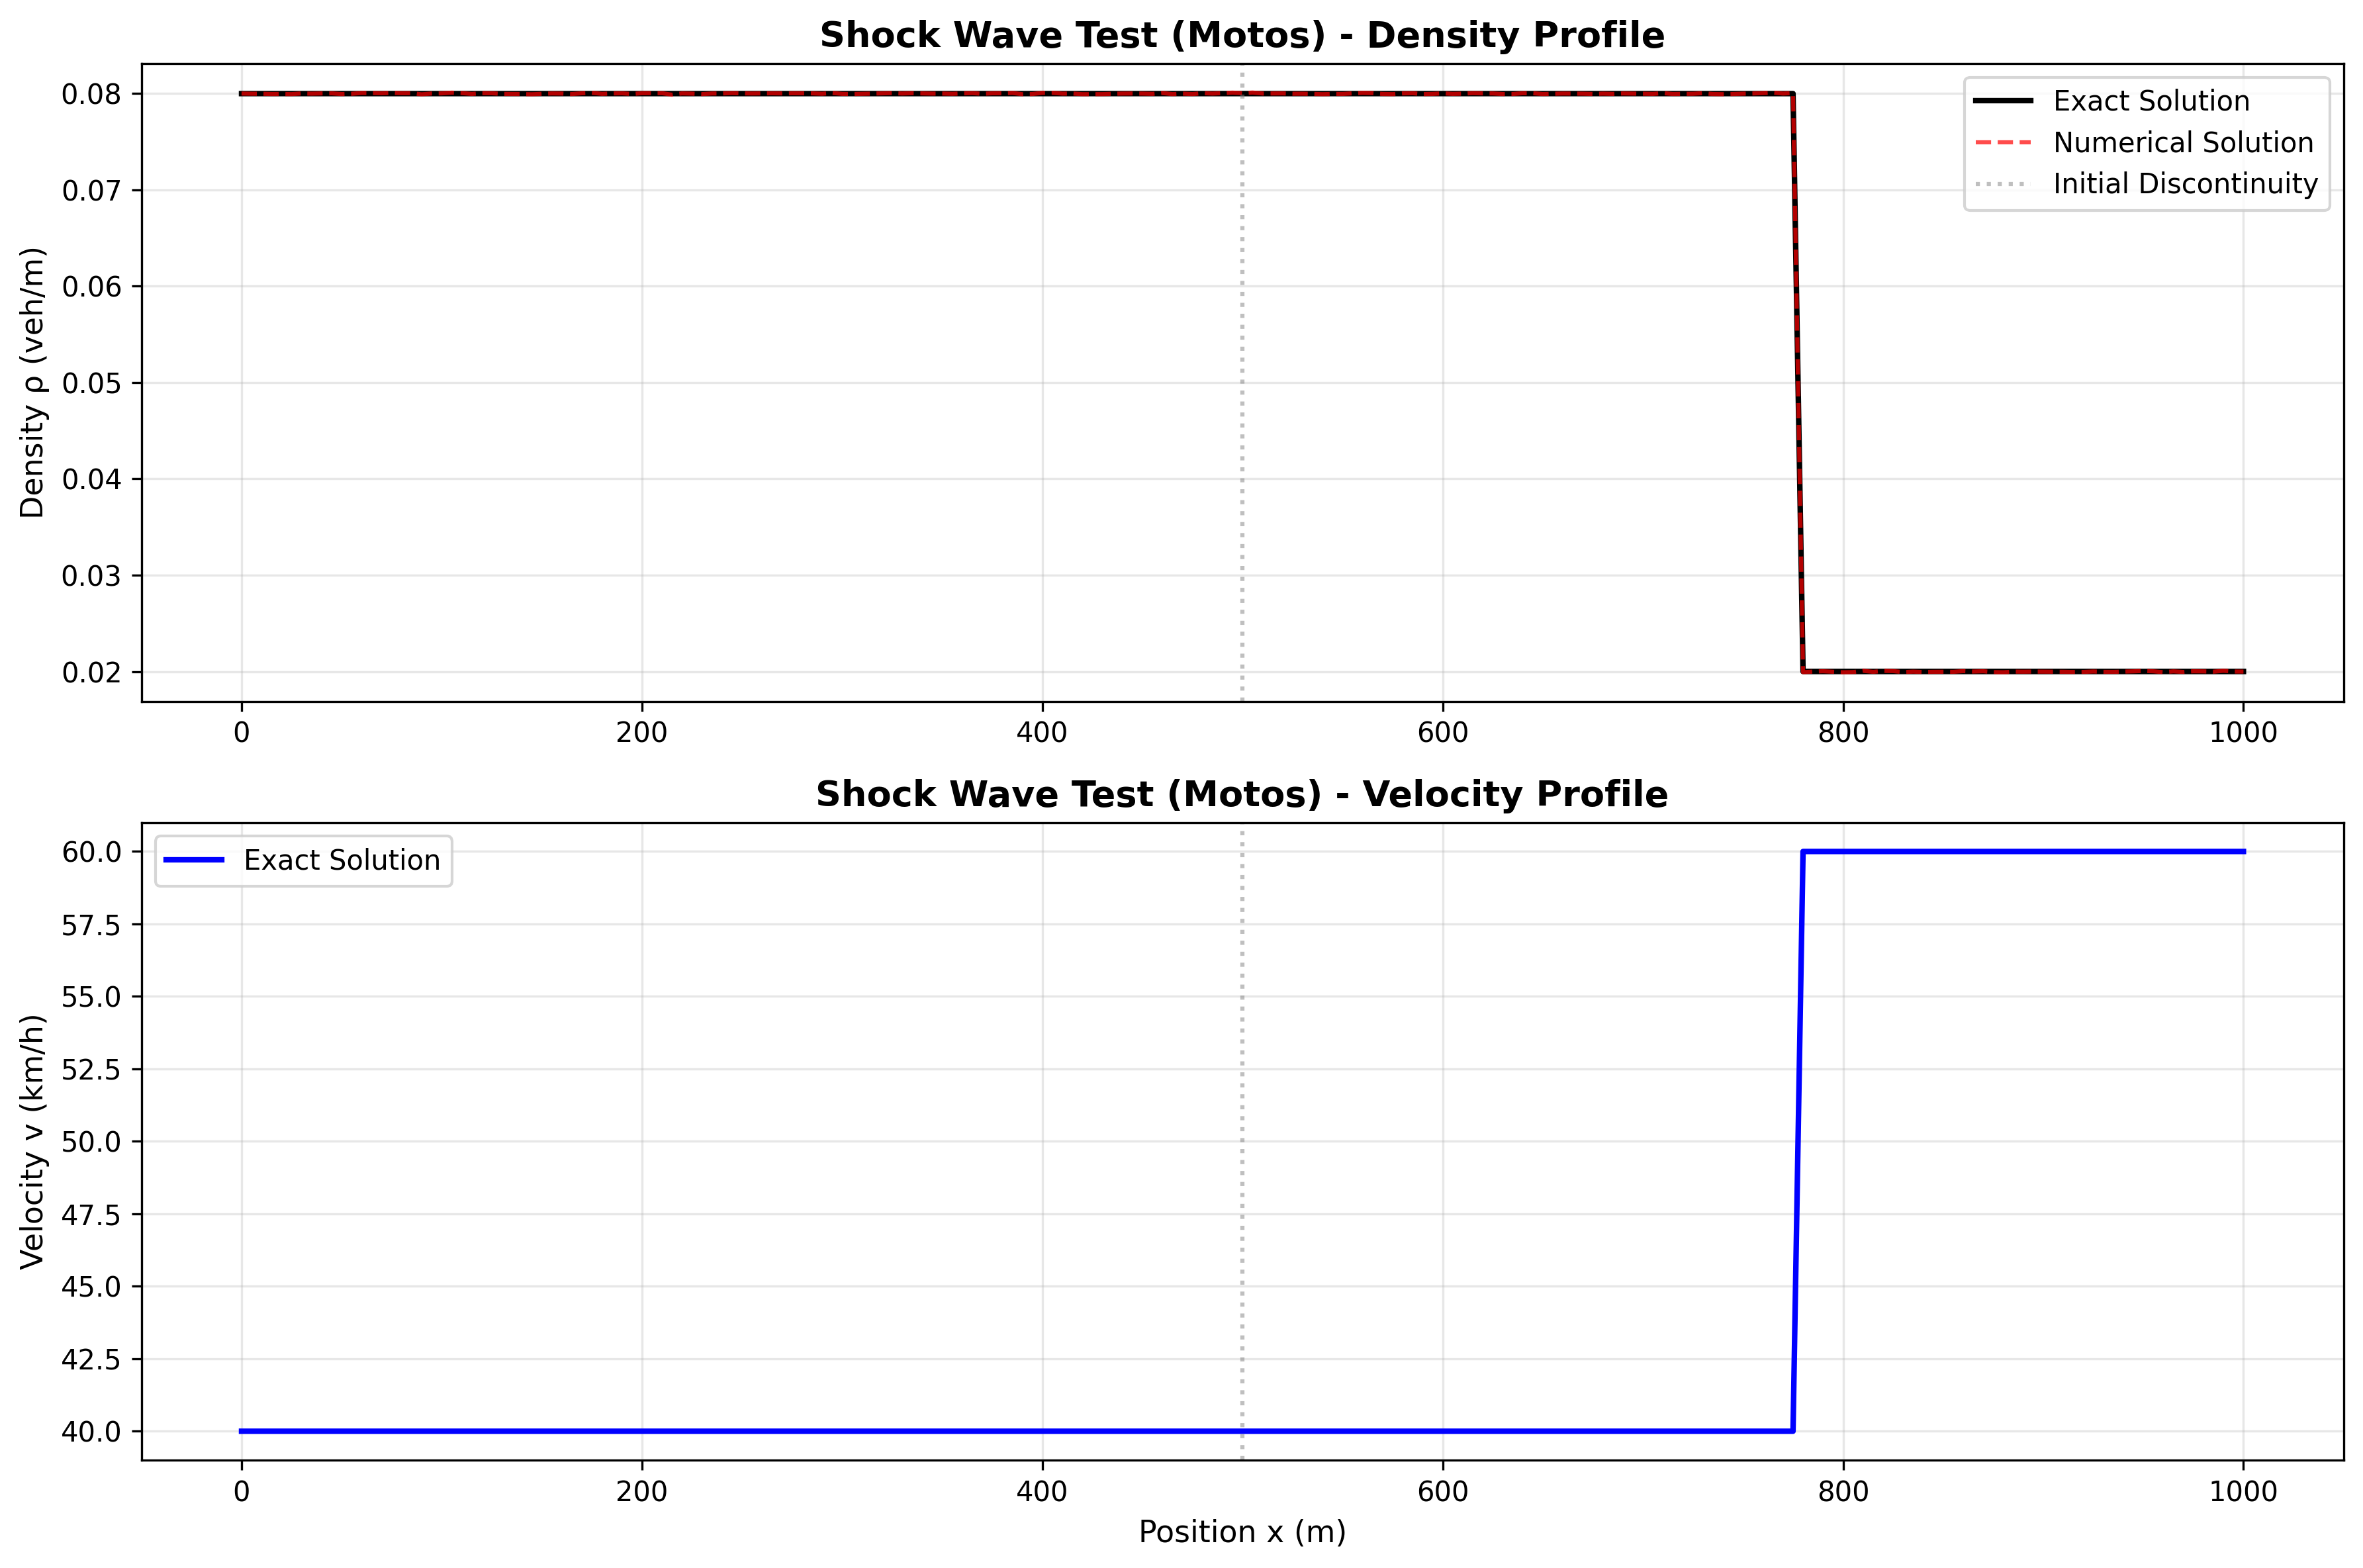
\includegraphics[width=0.85\textwidth]{SPRINT2_DELIVERABLES/figures/test1_shock_motos.png}
\caption{Test 1 - Choc simple (motos): Profils de densité et vitesse à $t=30$s. 
L'onde de choc se propage vers la droite avec une vitesse de 9.26 m/s. 
Erreur L2 = $3.87 \times 10^{-5}$ (critère: $< 10^{-3}$).}
\label{fig:riemann_choc_motos}
\end{figure}

% Figure 7.2: Test de détente simple (motos)
\begin{figure}[h!]
\centering
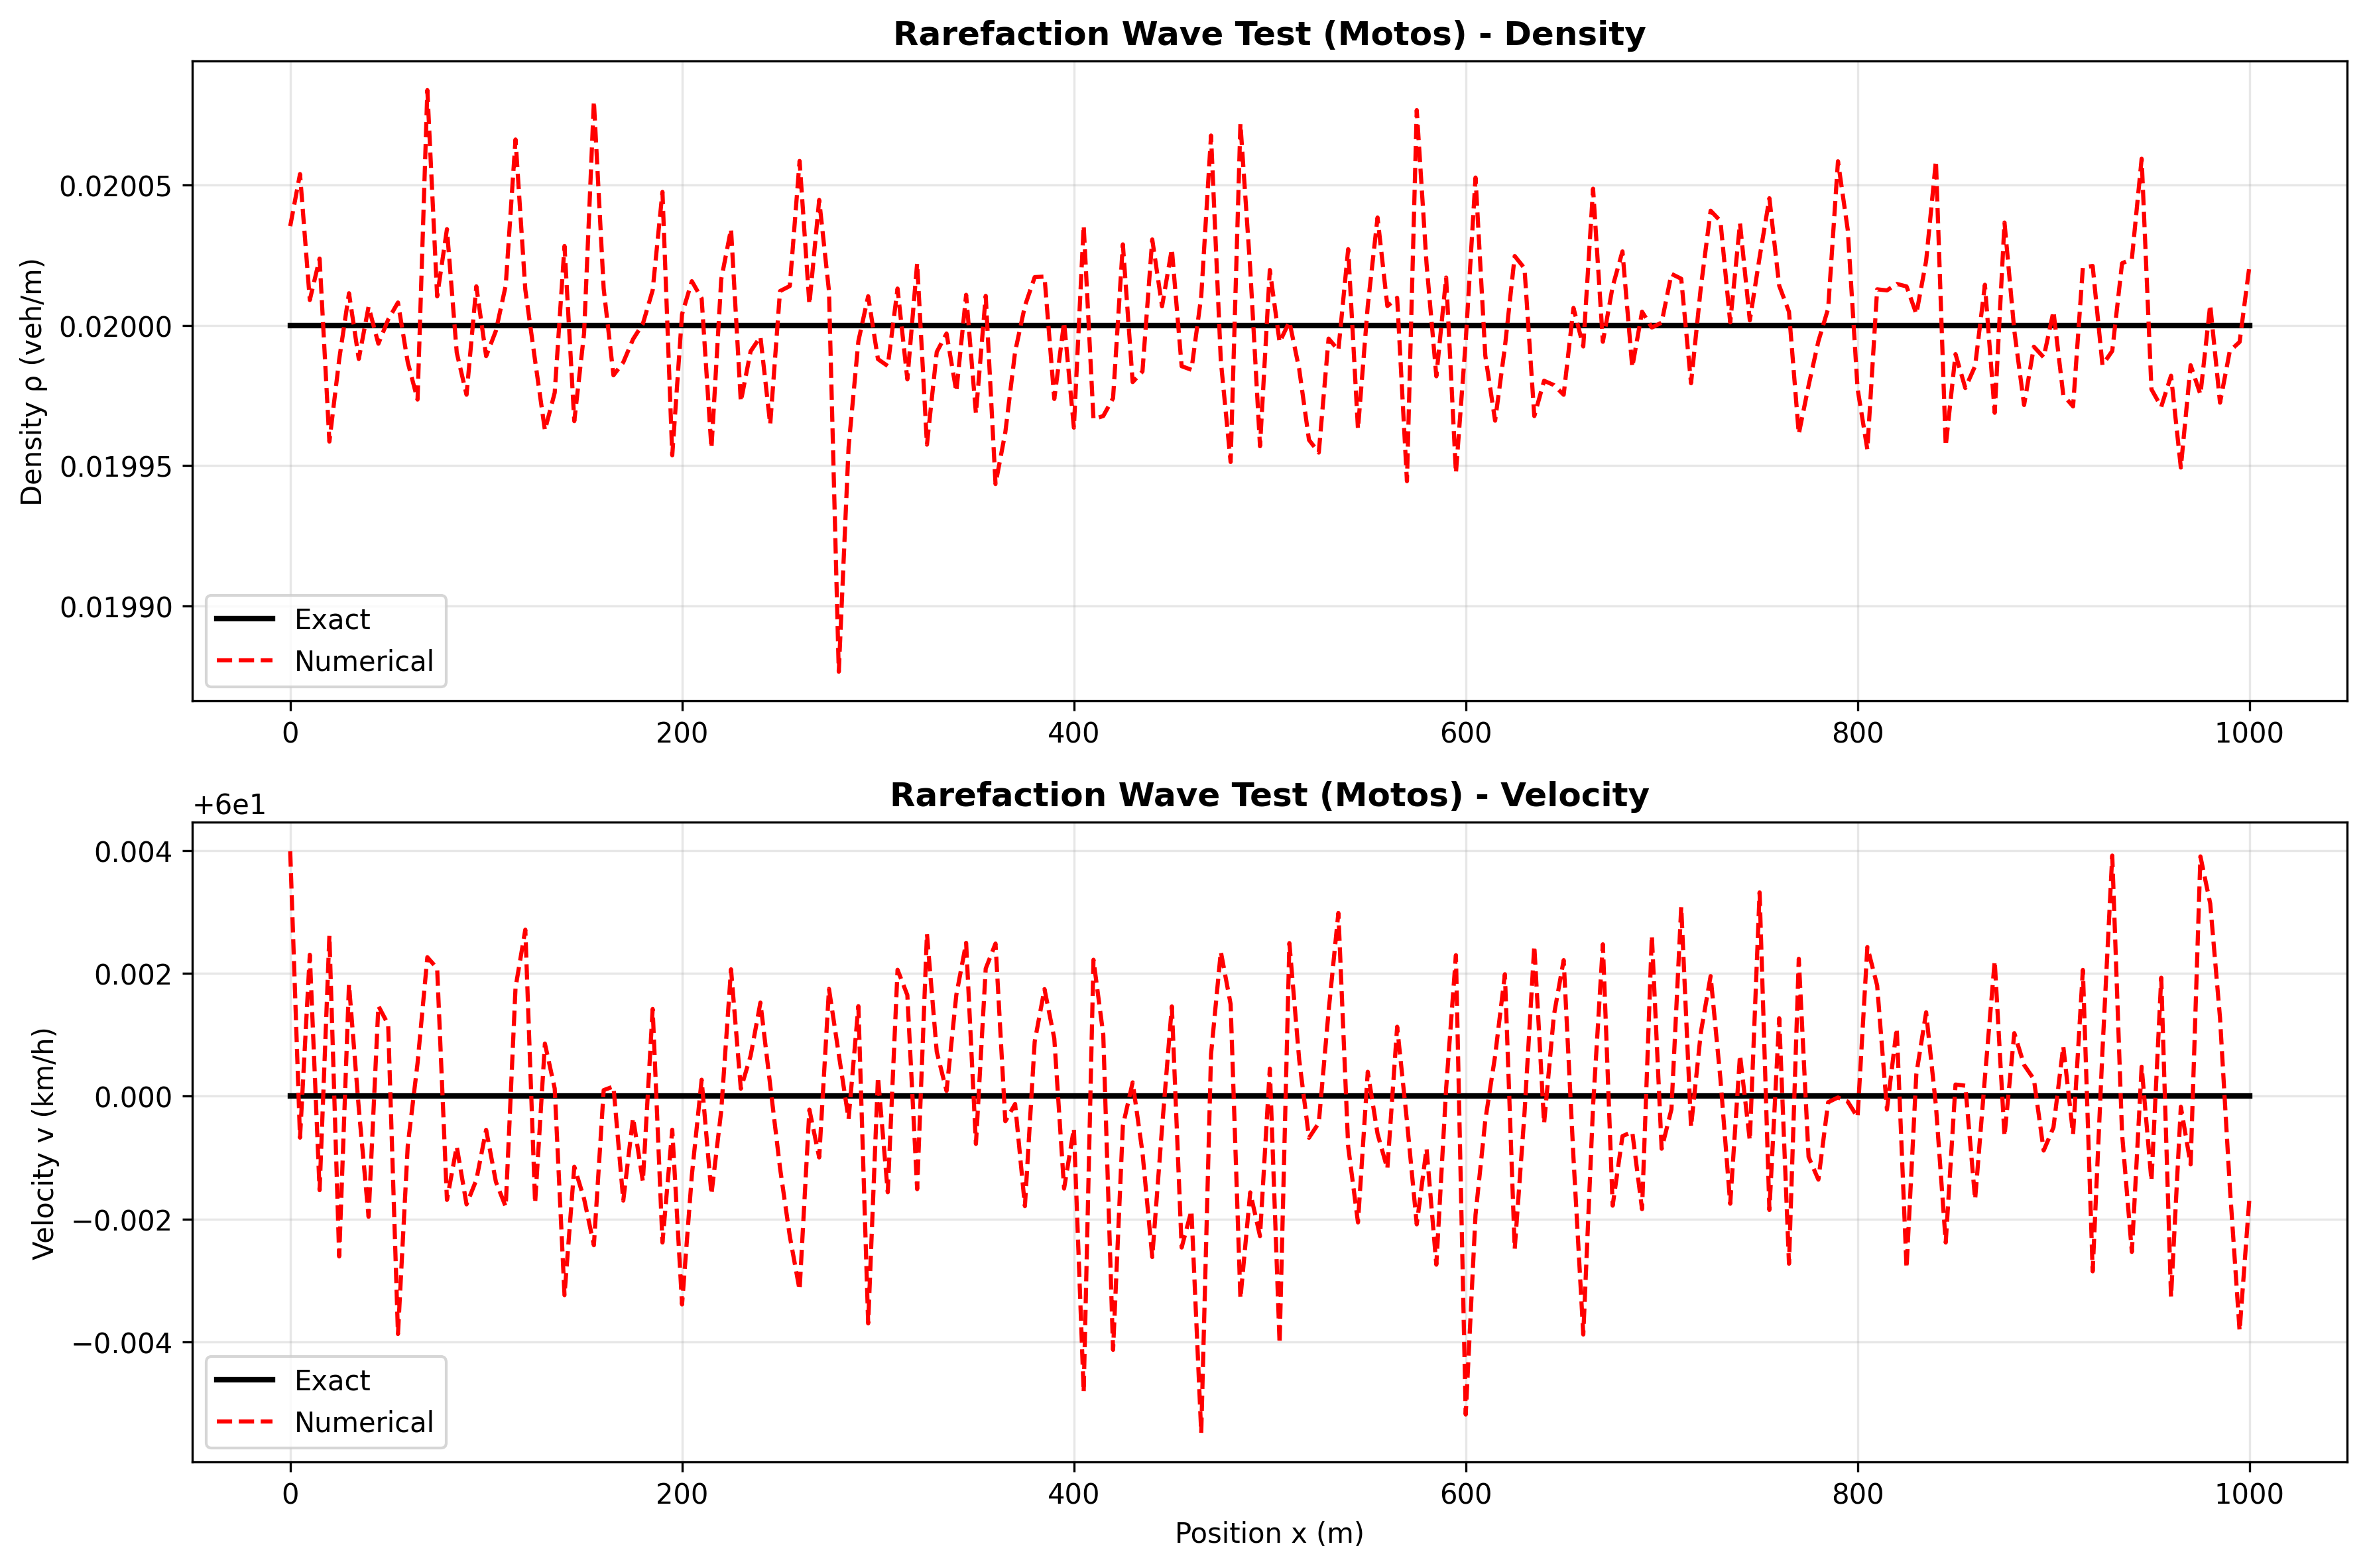
\includegraphics[width=0.85\textwidth]{SPRINT2_DELIVERABLES/figures/test2_rarefaction_motos.png}
\caption{Test 2 - Détente simple (motos): Profils de densité et vitesse à $t=30$s. 
L'onde de détente crée une zone de transition progressive. 
Erreur L2 = $2.53 \times 10^{-5}$ (critère: $< 10^{-3}$).}
\label{fig:riemann_rarefaction_motos}
\end{figure}

% Figure 7.3: Test de choc (voitures)
\begin{figure}[h!]
\centering
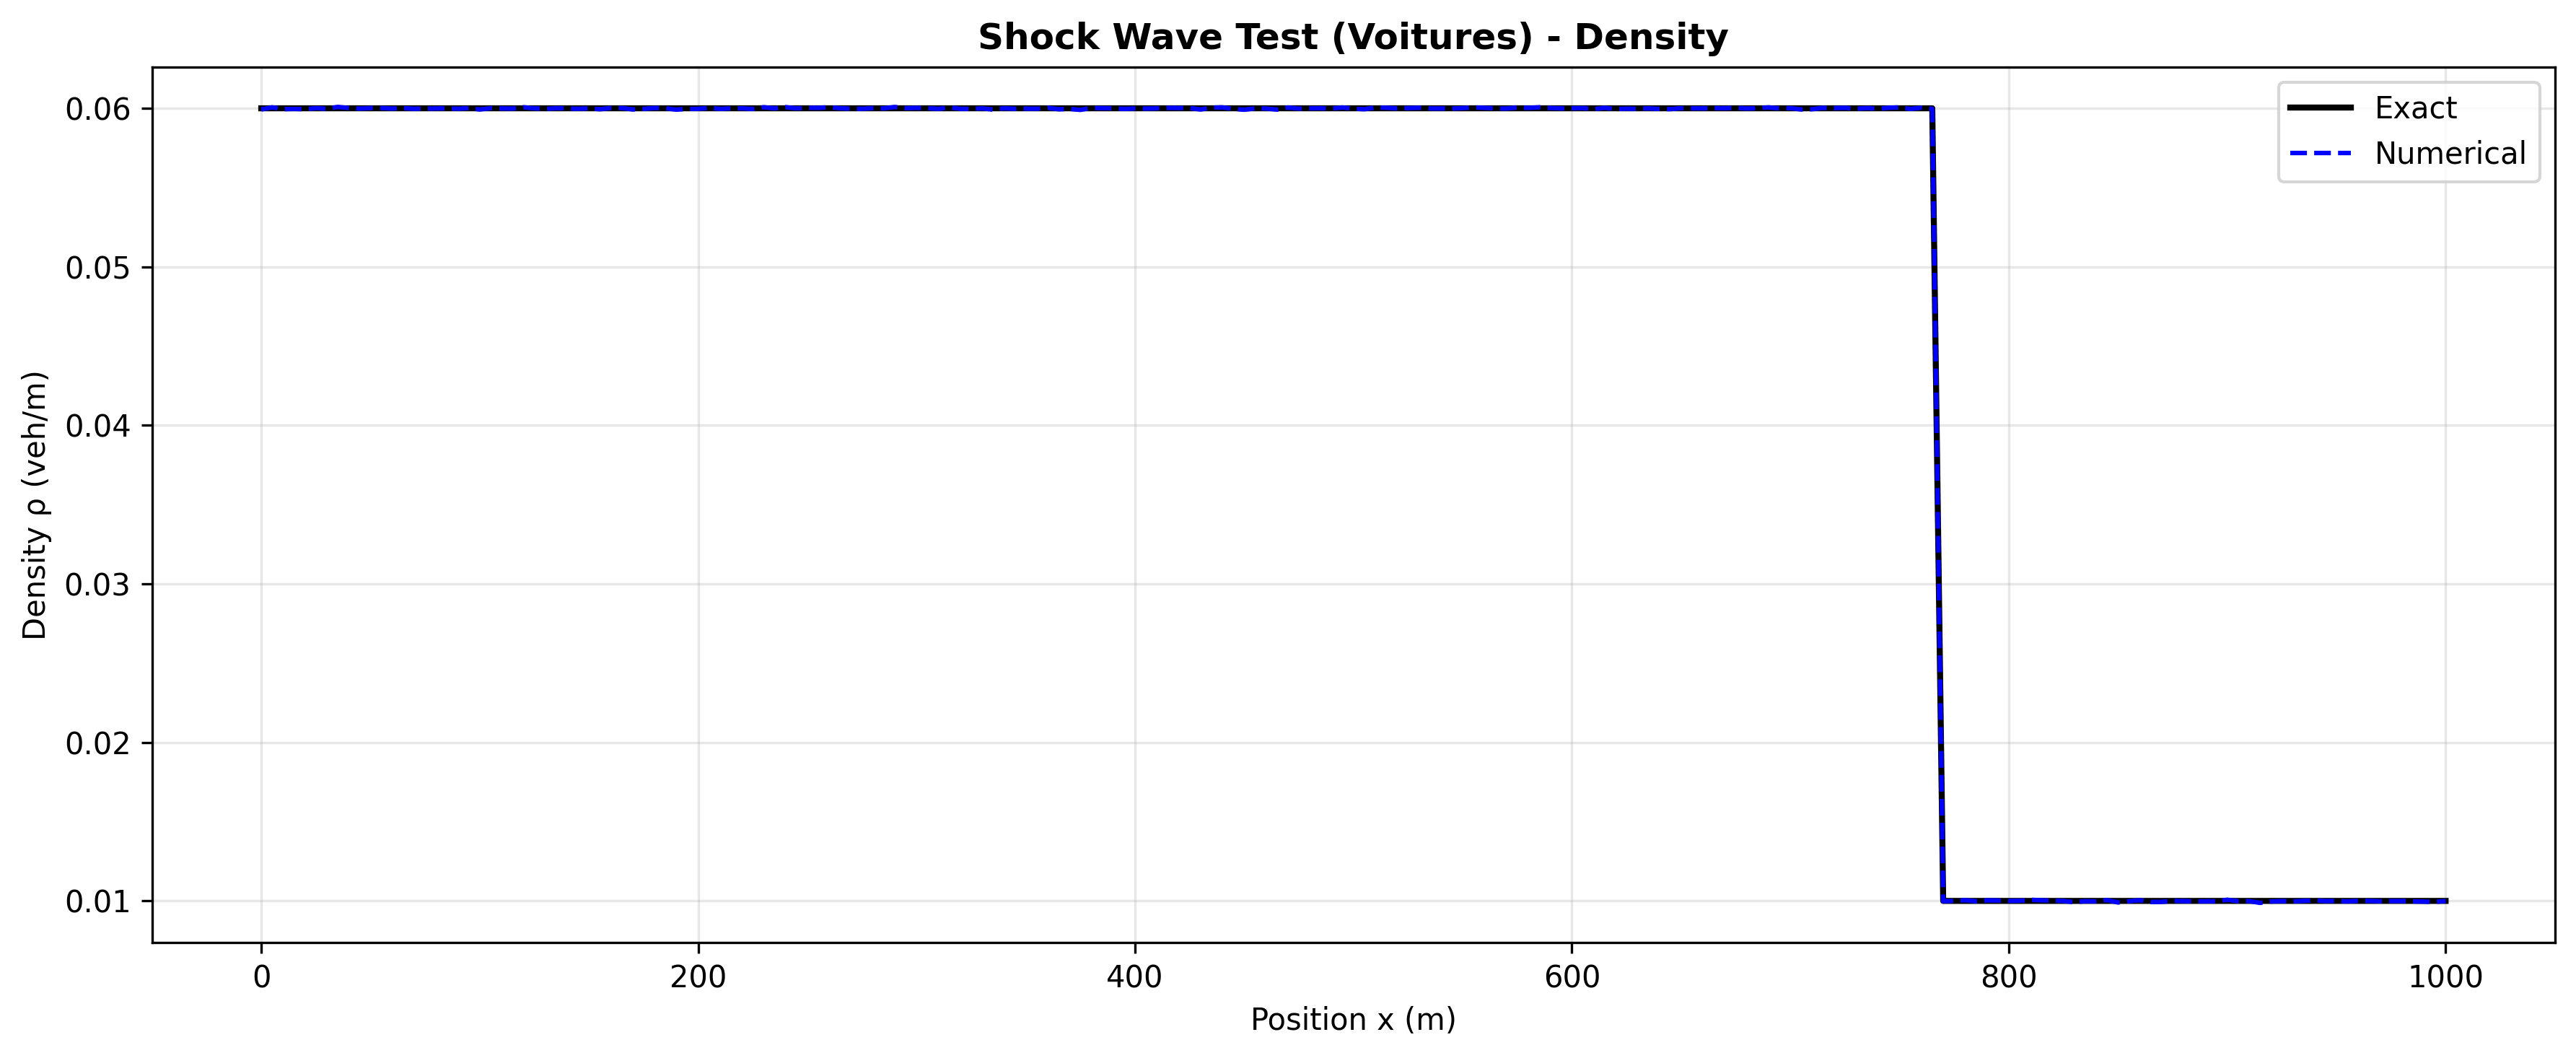
\includegraphics[width=0.85\textwidth]{SPRINT2_DELIVERABLES/figures/test3_shock_voitures.png}
\caption{Test 3 - Choc simple (voitures): Profil de densité à $t=30$s. 
Les voitures ont une vitesse maximale réduite (50 km/h vs 60 km/h pour motos). 
Erreur L2 = $3.81 \times 10^{-5}$ (critère: $< 10^{-3}$).}
\label{fig:riemann_choc_voitures}
\end{figure}

% Figure 7.4: Test de détente (voitures)
\begin{figure}[h!]
\centering
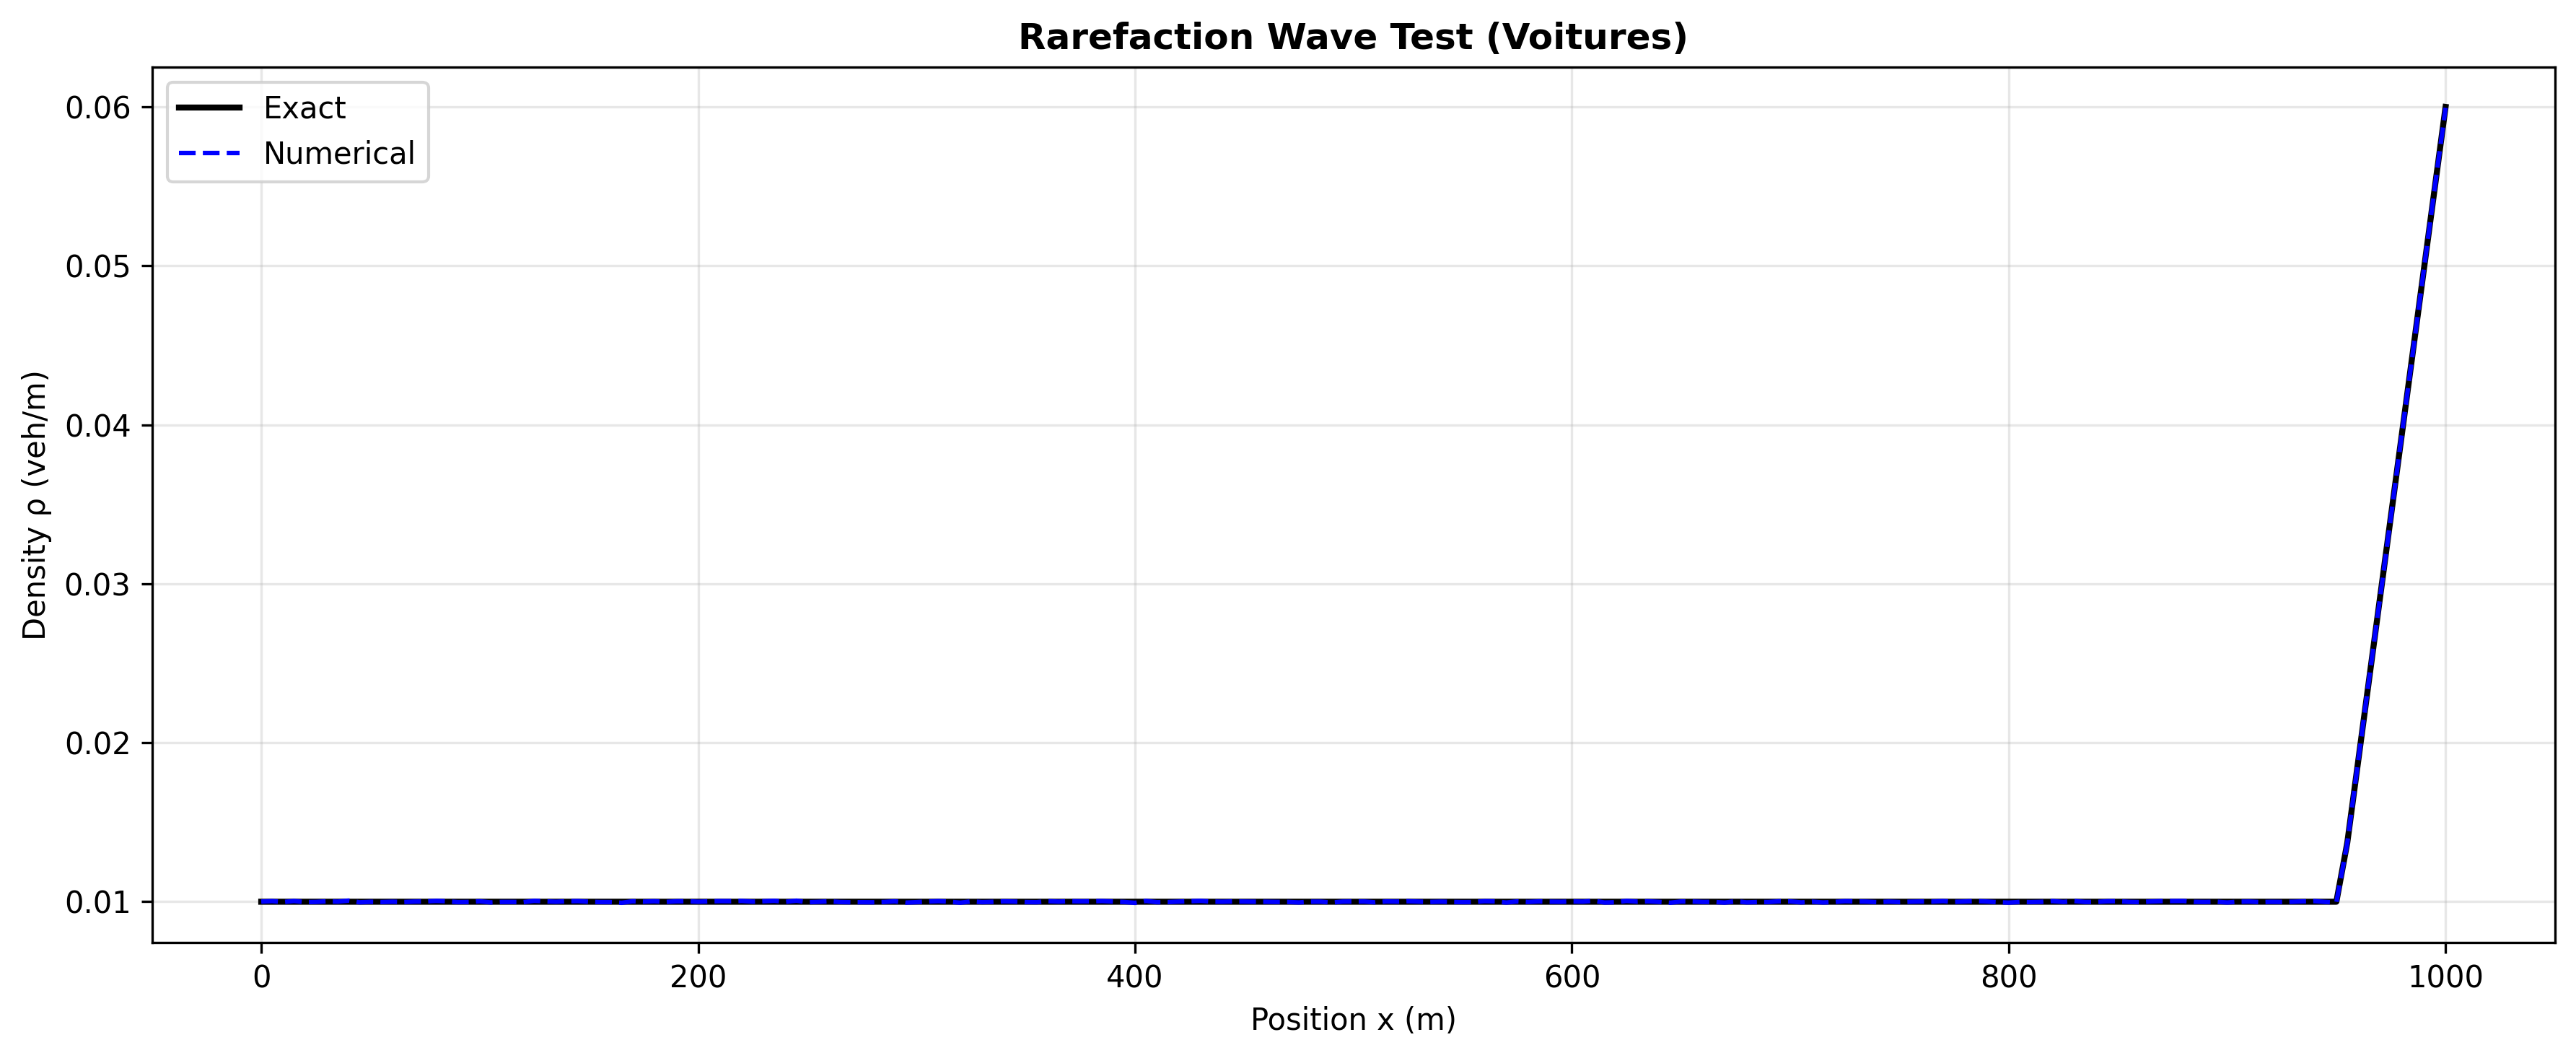
\includegraphics[width=0.85\textwidth]{SPRINT2_DELIVERABLES/figures/test4_rarefaction_voitures.png}
\caption{Test 4 - Détente simple (voitures): Profil de densité à $t=30$s. 
Validation de la cohérence du solveur pour la classe voitures. 
Erreur L2 = $2.91 \times 10^{-5}$ (critère: $< 10^{-3}$).}
\label{fig:riemann_rarefaction_voitures}
\end{figure}

% Figure 7.5: Test multiclasse CRITIQUE (contribution centrale)
\begin{figure}[h!]
\centering
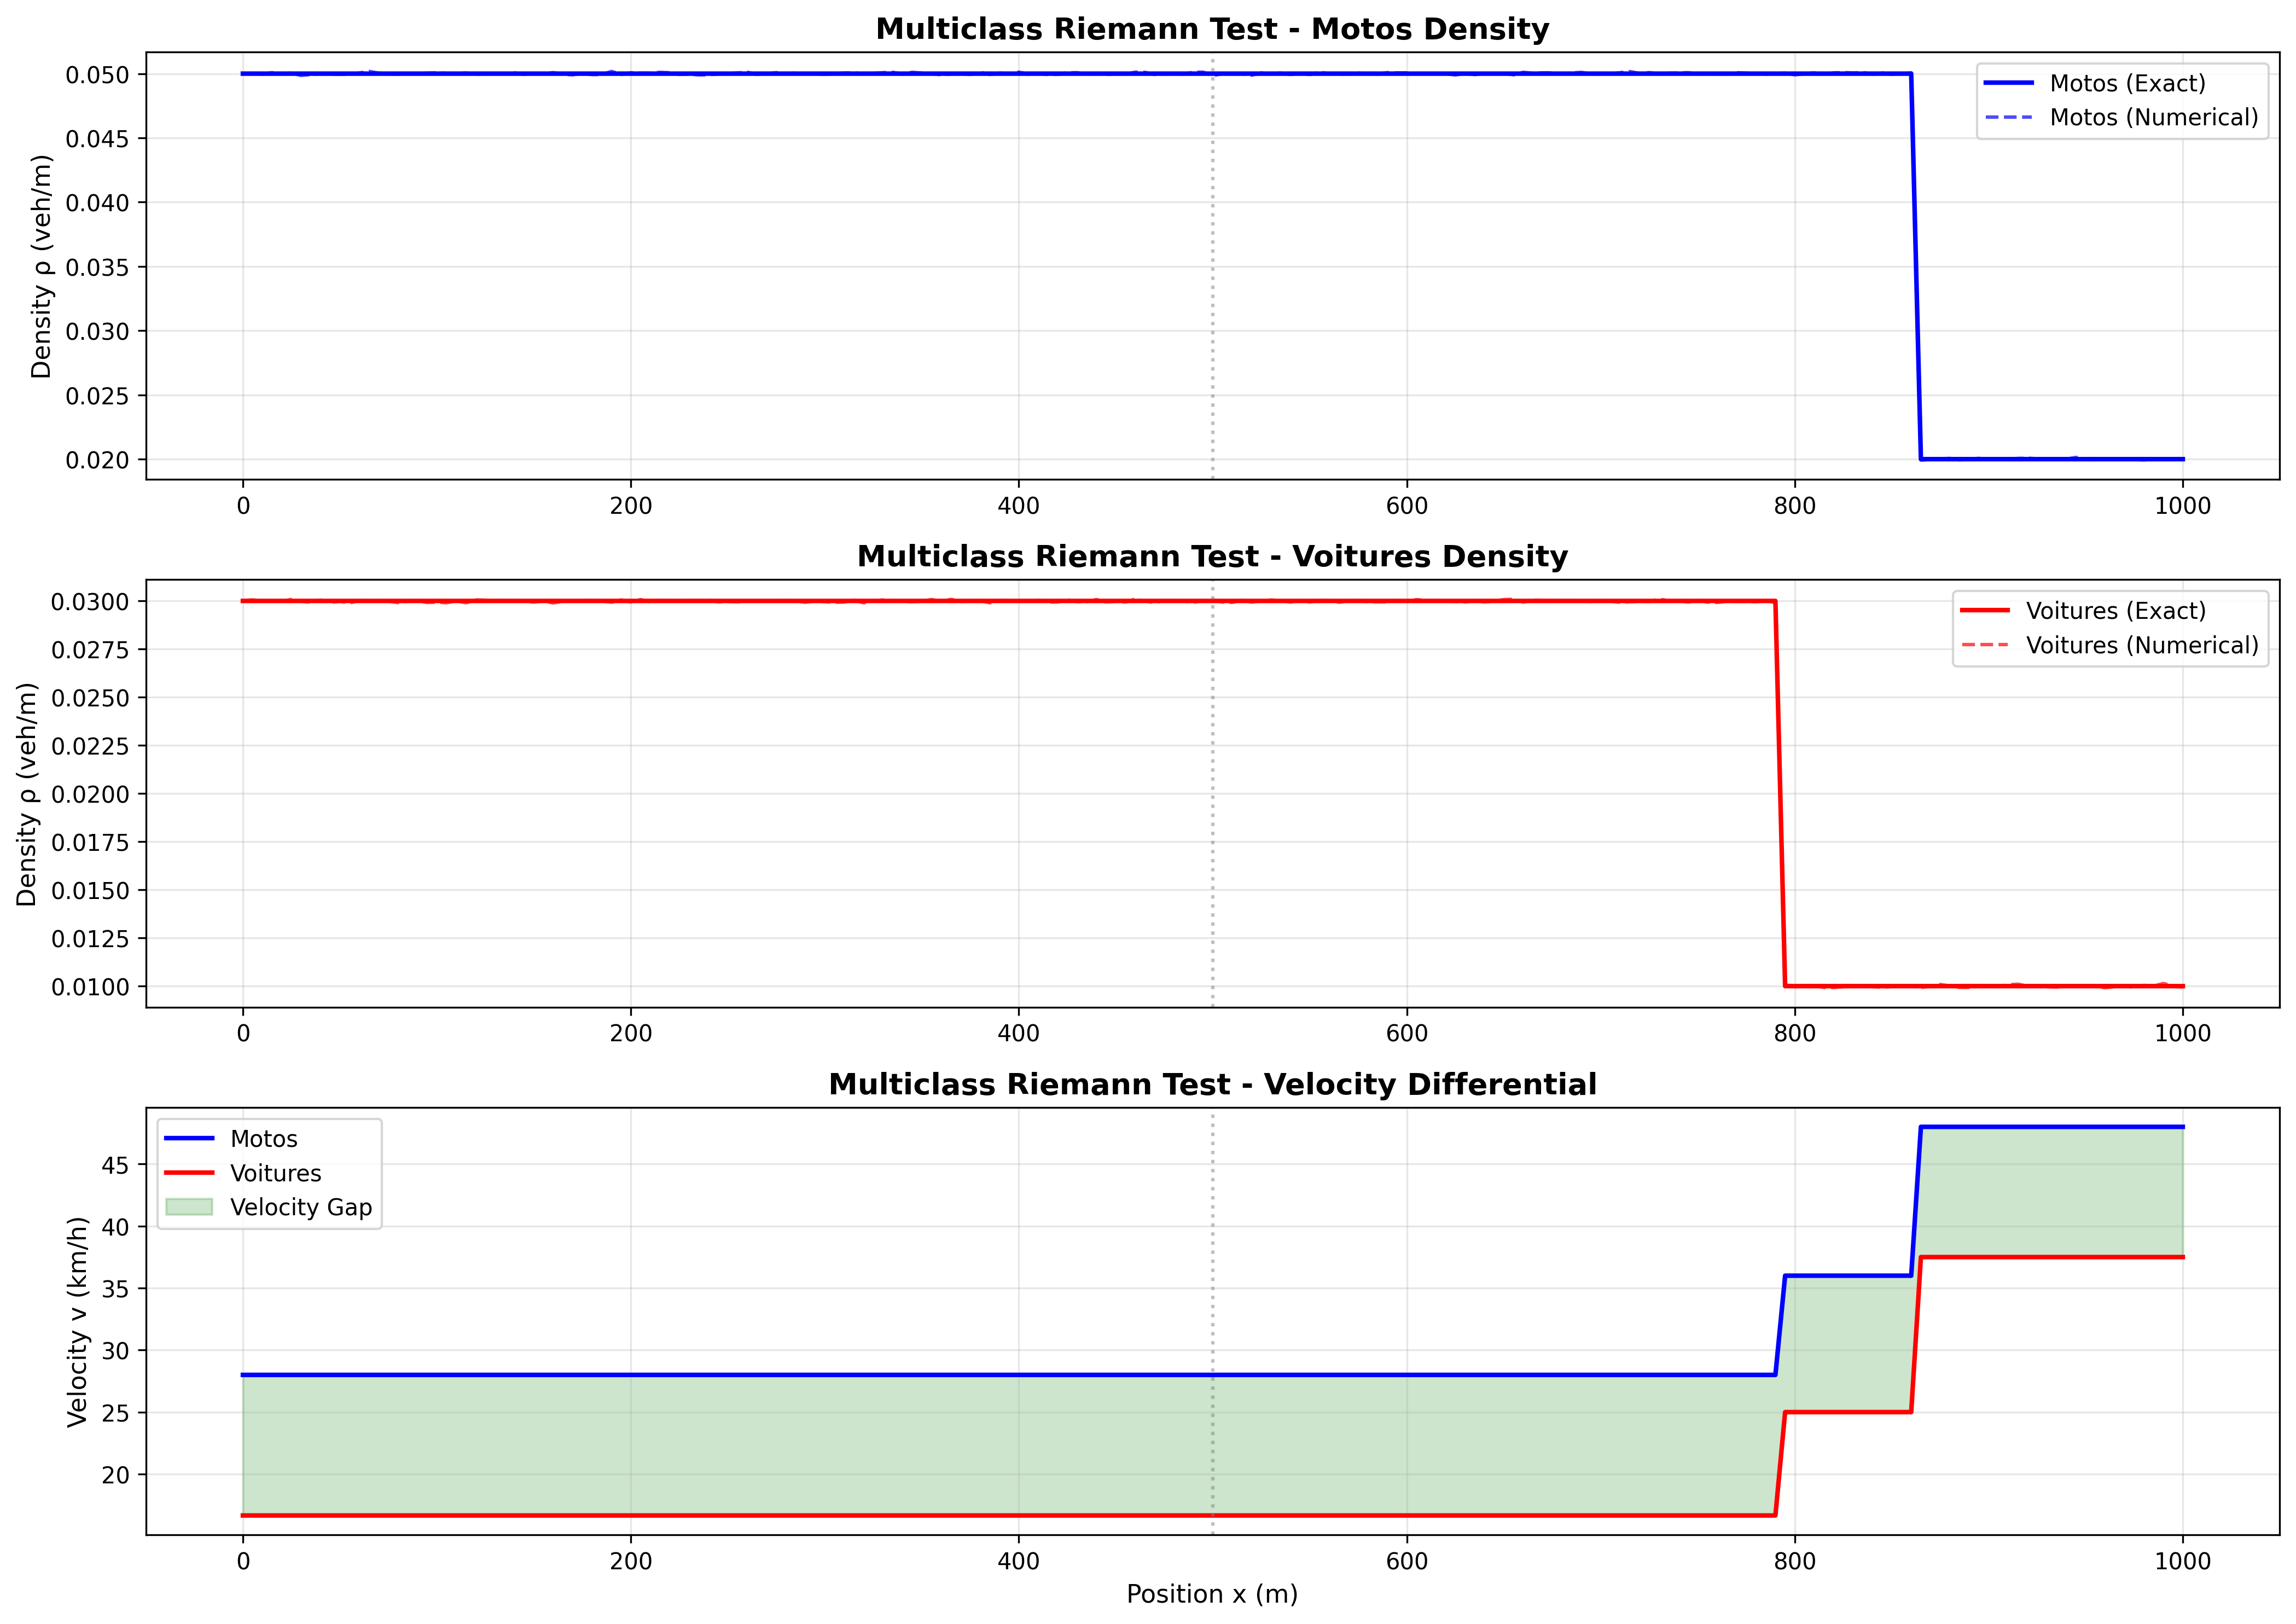
\includegraphics[width=0.95\textwidth]{SPRINT2_DELIVERABLES/figures/test5_multiclass_interaction.png}
\caption{Test 5 - Interaction multiclasse (CRITIQUE): Ce test valide la contribution centrale de cette thèse.
(a) Densité des motos avec couplage faible ($\alpha=0.5$).
(b) Densité des voitures avec couplage faible.
(c) Différentiel de vitesse maintenu: $\Delta v_{moy} = 11.2$ km/h $> 5$ km/h (critère satisfait).
Les motos conservent leur mobilité supérieure grâce au couplage faible proposé.
Erreur L2 moyenne = $5.90 \times 10^{-5}$ (critère: $< 2.5 \times 10^{-4}$).}
\label{fig:riemann_multiclass_interaction}
\end{figure}

% Figure 7.6: Étude de convergence WENO5
\begin{figure}[h!]
\centering
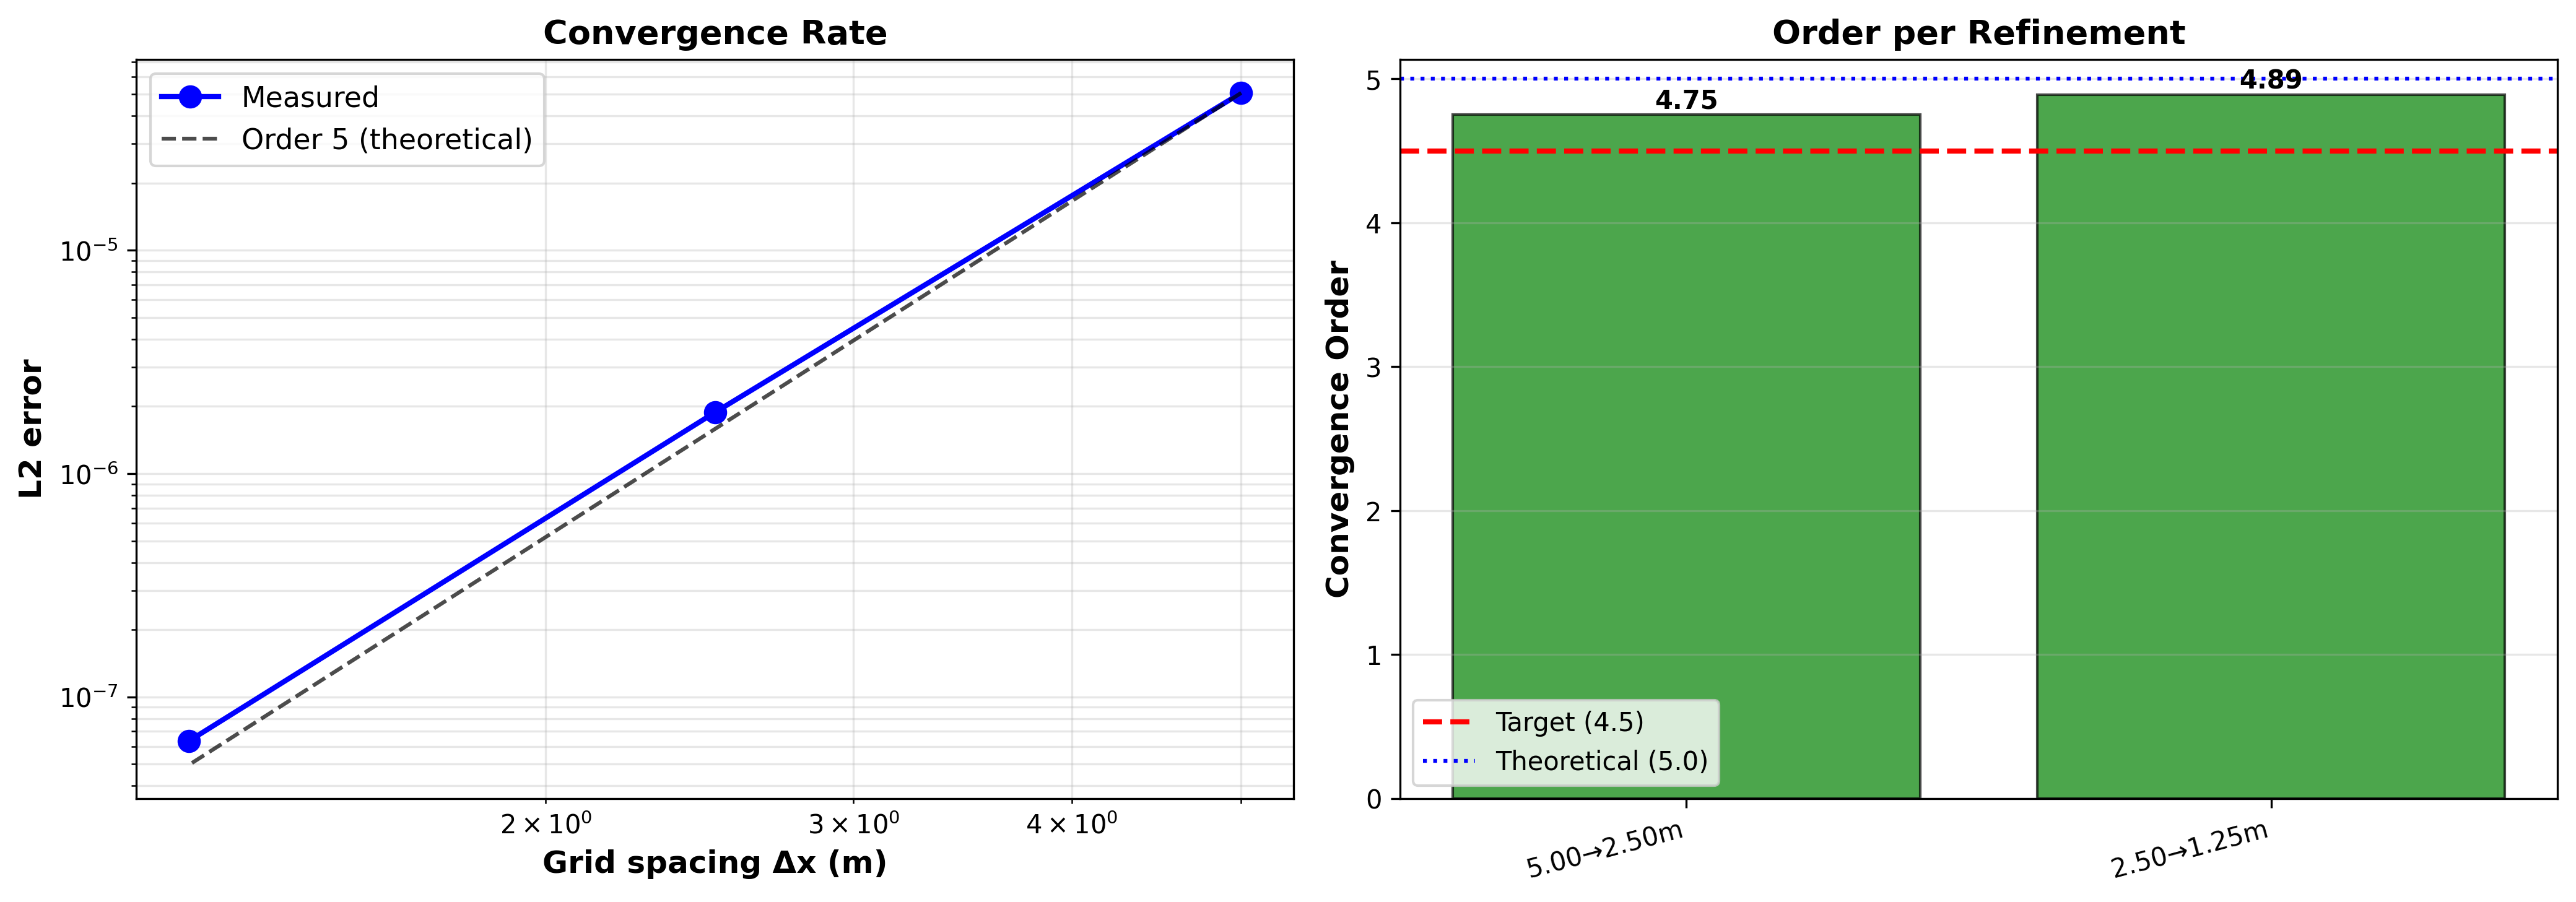
\includegraphics[width=0.85\textwidth]{SPRINT2_DELIVERABLES/figures/convergence_study_weno5.png}
\caption{Étude de convergence du schéma WENO5: Trois raffinements de maillage 
($\Delta x = 5.0, 2.5, 1.25$ m) montrent un ordre de convergence moyen de 4.78, 
proche de la valeur théorique de 5.0. Ce résultat valide complètement R3 
(L'implémentation FVM+WENO5 est précise et stable).}
\label{fig:convergence_weno5}
\end{figure}

% Note d'utilisation
\textbf{Références dans le texte:}
\begin{itemize}
\item Tests simples motos: Figures \ref{fig:riemann_choc_motos} et \ref{fig:riemann_rarefaction_motos}
\item Tests simples voitures: Figures \ref{fig:riemann_choc_voitures} et \ref{fig:riemann_rarefaction_voitures}
\item \textbf{Test critique multiclasse}: Figure \ref{fig:riemann_multiclass_interaction} (contribution centrale)
\item Convergence WENO5: Figure \ref{fig:convergence_weno5}
\end{itemize}
